\documentclass[../mathNotesPreamble]{subfiles}
\pgfplotsset{compat=newest}
\usepgfplotslibrary{statistics}

% Adapted from section 5.12.1 of pgfplots (v 1.18.1) documentation
%  \begin{center}
%    \begin{tikzpicture}
%      \begin{axis}[
%        width=0.75\linewidth, height=0.2\linewidth,
%        ymajorticks=false]
%        \addplot+ [boxplot]
%          table [row sep=\\,y index=0] {
%            data\\
%            1\\ 2\\ 1\\ 5\\ 4\\ 10\\
%            7\\ 10\\ 9\\ 8\\ 9\\ 9\\ 19\\
%          };
%      \end{axis}
%    \end{tikzpicture}
%  \end{center}

\providecommand{\relscalefact}{1.4}
\begin{document}
\relscale{\relscalefact}
  \section{3.5: Using Boxplots for Displaying Summaries}

  \begin{defn*}
    A \textbf{boxplot} is a graphical tool for visualizing a distribution. Boxplots can be useful for comparing multiple distributions. In a box plot:
    \begin{itemize}
      \item The left edge of the box represents $Q_1$
      \item The vertical line inside the box represents the median ($Q_2$)
      \item The right edge of the box represents $Q_3$
      \item Lines extending past the edges of the box are called whiskers. The whiskers extend to the most extreme values that are not \emph{potential} outliers.
    \end{itemize}
  \end{defn*}
  \vspace*{\stretch{1}}

  \begin{center}
    \begin{tikzpicture}
      \begin{axis}[
        axis lines=center,
        axis line style={black,->},
        xmin=2.15, xmax=2.41,
        ymin=0, ymax=4,
        ymajorticks=false,
        width=0.875\linewidth, height=0.3\linewidth,
        ticklabel style={font=\normalsize,inner sep=0.5pt,fill=white,opacity=1.0, text opacity=1}]
        \foreach \price/\freq in {
          2.17/1,
          2.19/3,
          2.24/1,
          2.27/1,
          2.29/3,
          2.30/1,
          2.38/2
          }{
          \foreach \x in {1,...,\freq}
            \addplot[soldot, mark size=2pt] coordinates{(\price,\x)};
          }
      \end{axis}
    \end{tikzpicture}
    \vspace*{\stretch{1}}

    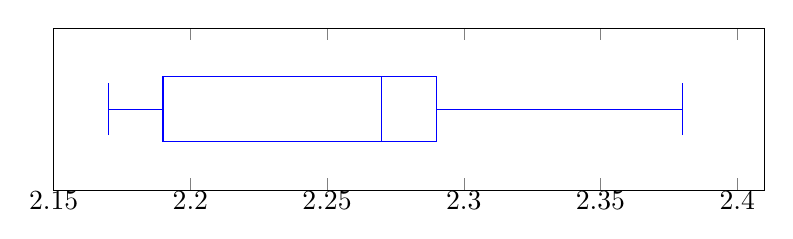
\begin{tikzpicture}[declare function={Y=1;}] %Using "Y" to control the height of the boxplot
      \begin{axis}[
        xmin=2.15, xmax=2.41,
        ymin=1-Y, ymax=1+Y,
        ymajorticks=false,
        width=0.875\linewidth, height=0.3\linewidth,
        ticklabel style={font=\normalsize,inner sep=0.5pt,fill=white,opacity=1.0, text opacity=1}]
        \addplot+ [boxplot]
          table [row sep=\\,y index=0] {
            data\\
            2.17\\ 2.19\\ 2.19\\ 2.19\\ 2.24\\
            2.27\\ 2.29\\ 2.29\\ 2.29\\ 2.30\\ 2.38\\
          };
      \end{axis}
    \end{tikzpicture}
  \end{center}
%  \vspace*{\stretch{1}}
  \pagebreak

  \begin{defn*}
    \textbf{Potential outliers} are any values that are
    \begin{itemize}
      \item less than $Q_1-1.5IQR$
      \item more than $Q_3+1.5IQR$
    \end{itemize}
    These values are the left and right limits. They are also known as the \emph{fences}.
  \end{defn*}

  \begin{ex*}
    Using the ``airtemp'' dataset in StatCrunch, generate the boxplots for the daily maximum temperature in San Francisco and Provo. Compute the left and right limits. Are they included in the plots?
  \end{ex*}

  \begin{center}
    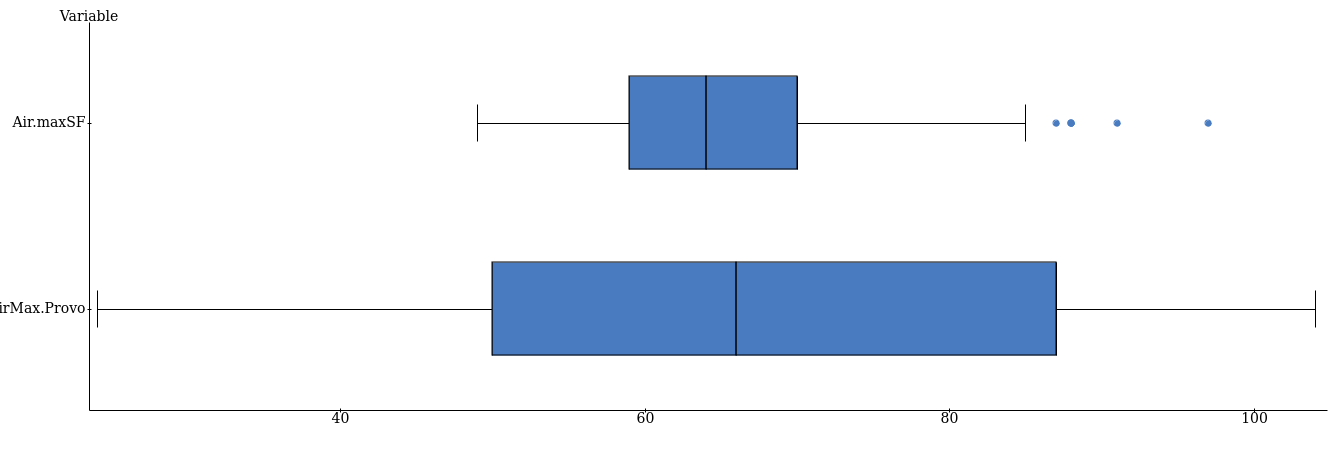
\includegraphics[width=0.925\linewidth]{images/math211_sf_provo_temp_boxplots}
  \end{center}
  \vspace*{\stretch{1}}

  \begin{defn*}
    The \textbf{five number summary} is
    \begin{center}
       the minimum, $Q_1$, the median, $Q_3$, the maximum
    \end{center}
  \end{defn*}

  \pagebreak
\end{document}
